\section{Evaluation}\label{sec:evaluation}

\subsection{Setup}\label{sec:setup}

\paragraph{One frozen checkpoint.} Every experiment in this section runs on one checkpoint that we froze before the first run: the controller, trainer, and harness code, the six patched engine files, the two calibration files, the factory drafters, the target weights, the prompt pools, the seeds, and the software environment, each recorded by hash (\cref{app:manifest}). The simulator of \cref{sec:heldout} reads the same frozen calibration file.

\paragraph{Workload.} Each run serves three phases on one H100 GPU: 200 chat requests at concurrency 16 (phase A1), then 16{,}000 unique requests from a new domain at concurrency 256, which saturate the GPU for \nv{bdur.min}--\nv{bdur.max}\,s (phase B), then 200 different chat requests (phase A2). The three scenarios are Qwen3-8B with code in B, Qwen3-8B with Chinese in B, and Qwen3-30B-A3B with code in B. Decoding is greedy, outputs stop naturally or at 512 tokens, and the B prompts were never seen during calibration. Every policy except the production reference reserves the trainer's memory (18\,GB for Qwen3-8B and 5\,GB for the MoE target), and every such policy that loads a drafter also runs the export path.

\paragraph{Policies.} \pol{Production} runs the factory drafter with speculation always on, without export or memory reserve, as deployed today. \pol{Static} does the same under the evaluation's engine configuration and is the reference for all differences. \pol{Plain} serves without a drafter. \pol{Switch} applies \cref{eq:switch} with the domain's frontier and never trains. \pol{Threshold} turns speculation off whenever the server is saturated and trains at duty 0.5 whenever TPOT is within the SLO, i.e., the idle-time rule of OSD \citep{liu2024osd} combined with a load threshold. \pol{Always} trains at duty 0.5 from the first request and swaps drafters after 100, 200, 400, \dots{} requests. \pol{Informed} trains at duty 0.5 from the moment phase B starts until it has learned from 800 requests, swapping at 100, 200, 400, and 800; we chose its stopping point from the learning curves of \cref{fig:motivation}c, so it is a reference that knows when to stop rather than a deployable policy. \pol{Full} is the controller of \cref{sec:method}. \pol{Always} and \pol{Informed} never turn speculation off (\cref{app:policies}).

\paragraph{Repetitions and metrics.} Every policy runs three times per scenario. Repetition $r$ fixes the prompt order of all phases and the trainer's random seed, so within a repetition all policies serve the same request sequence, and we report paired differences as mean $\pm$ standard deviation over the three pairs. The main metric is output throughput during phase B; we also report TPOT and the throughput of the whole run. The \nv{n.runs} runs used \nv{gpuh} GPU-hours on \nv{hosts} nodes of the same type; the coefficient of variation of B throughput was at most \nv{cv.static.max}\% for the static policies.

\subsection{The best policy differs by scenario}\label{sec:results}

\begin{table*}[t]
\caption{Phase-B (saturated) throughput relative to \pol{Static}: paired mean $\pm$ standard deviation over three repetitions, in percent. Parentheses give mean throughput as a fraction of the best policy in that scenario (bold); the \pol{Static} row gives absolute throughput. The last column is the smallest fraction over the three scenarios.}
\label{tab:main}
\centering\small
% generated by code/specsched/paper_assets.py -- do not edit by hand
\begin{tabular}{@{}lcccc@{}}
\toprule
Policy & 8B code & 8B Chinese & MoE code & Worst case\\
\midrule
Production speculation & $+2.2$\,$\pm$0.9 \,{\scriptsize(0.854)} & $+1.8$\,$\pm$0.8 \,{\scriptsize(0.517)} & $+1.0$\,$\pm$0.1 \,{\scriptsize(0.923)} & 0.517 \\
Static speculation & 14{,}282 tok/s \,{\scriptsize(0.835)} & 8{,}526 tok/s \,{\scriptsize(0.508)} & 13{,}859 tok/s \,{\scriptsize(0.915)} & 0.508 \\
Plain decoding & $+18.1$\,$\pm$0.9 \,{\scriptsize(0.986)} & \textbf{\boldmath $+97.0$\,$\pm$1.4 \,{\scriptsize(1.000)}} & $-46.1$\,$\pm$0.1 \,{\scriptsize(0.493)} & 0.493 \\
\addlinespace[2pt]
Switch only & $+12.9$\,$\pm$2.5 \,{\scriptsize(0.943)} & $+90.9$\,$\pm$2.2 \,{\scriptsize(0.969)} & $-0.3$\,$\pm$0.3 \,{\scriptsize(0.912)} & 0.912 \\
Threshold rule & $+14.8$\,$\pm$0.8 \,{\scriptsize(0.959)} & $+86.9$\,$\pm$4.7 \,{\scriptsize(0.949)} & $-46.0$\,$\pm$0.0 \,{\scriptsize(0.494)} & 0.494 \\
TIDE-style triggers & $+13.8$\,$\pm$3.5 \,{\scriptsize(0.950)} & $+54.5$\,$\pm$3.6 \,{\scriptsize(0.784)} & $+6.0$\,$\pm$4.0 \,{\scriptsize(0.970)} & 0.784 \\
\addlinespace[2pt]
Always train & $+2.4$\,$\pm$1.9 \,{\scriptsize(0.855)} & $-1.2$\,$\pm$0.7 \,{\scriptsize(0.502)} & $-3.6$\,$\pm$0.3 \,{\scriptsize(0.882)} & 0.502 \\
Informed schedule & \textbf{\boldmath $+19.7$\,$\pm$0.5 \,{\scriptsize(1.000)}} & $+13.8$\,$\pm$0.4 \,{\scriptsize(0.578)} & \textbf{\boldmath $+9.3$\,$\pm$0.7 \,{\scriptsize(1.000)}} & 0.578 \\
\rowcolor{resultgraylight}Full controller & $+18.0$\,$\pm$1.6 \,{\scriptsize(0.985)} & $+87.7$\,$\pm$8.5 \,{\scriptsize(0.953)} & $+8.0$\,$\pm$0.4 \,{\scriptsize(0.988)} & \textbf{0.953} \\
\bottomrule
\end{tabular}

\end{table*}

\begin{figure*}[t]
\centering
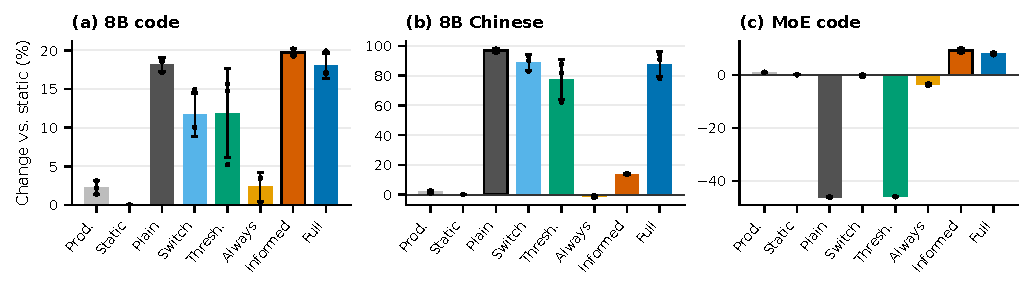
\includegraphics[width=\linewidth]{figures/fig4_policies.pdf}
\caption{Phase-B throughput change relative to \pol{Static} per repetition (dots), with the paired mean and standard deviation (bars). The best policy in each scenario has a black outline. Prod.: \pol{Production}; Thresh.: \pol{Threshold}.}
\label{fig:policies}
\end{figure*}

Table~\ref{tab:main} and Figure~\ref{fig:policies} show the frozen matrix. The best policy is \pol{Plain} for Qwen3-8B Chinese and \pol{Informed} for both code scenarios, and every policy other than \pol{Full} falls well short in at least one scenario. \pol{Plain} and \pol{Threshold} lose about half of the MoE throughput, because they turn speculation off where it is still \nv{fr.moe.n0.c256}$\times$ faster than plain decoding. \pol{Informed} keeps speculating on Chinese and reaches only \nv{zh.informed.r} of \pol{Plain}. \pol{Switch}, which never trains, is the most robust alternative but still falls \nv{switch.worstshort}\% short on MoE. \pol{Full} is the only policy within 5\% of the best in every scenario (worst case \nv{full.worst}). Against \pol{Static} it raises phase-B throughput by \nv{code.full.d}$\pm$\nv{code.full.sd}\%, \nv{zh.full.d}$\pm$\nv{zh.full.sd}\%, and \nv{moe.full.d}$\pm$\nv{moe.full.sd}\%, with the same sign in every repetition, and over the whole run it is \nv{code.full.session}\%, \nv{zh.full.session}\%, and \nv{moe.full.session}\% faster than \pol{Production}.

\subsection{Which lever the controller pulls}\label{sec:levers}

\begin{table*}[t]
\caption{What \pol{Full} did during phase B (means over three runs): fraction of time with speculation on, mean duty cycle, drafter swaps, acceptance length at the start and end of B, tokens trained over the whole run, and the decisions of the training tests, as a share of one-second ticks (shares below 5\% omitted).}
\label{tab:behaviour}
\centering\small
% generated by code/specsched/paper_assets.py -- do not edit by hand
\begin{tabularx}{\linewidth}{@{}lccccc>{\raggedright\arraybackslash}X@{}}
\toprule
Scenario & Spec.\ on & Duty & Swaps & Acceptance & Train tok.\ (M) & Decisions during the saturated phase (share of 1\,s ticks)\\
\midrule
8B code & 100\% & 0.067 & 3 & 2.50$\to$2.66 & 0.64 & no training (value $\le 0$) 77\%, train (value $>0$) 10\%, converged 10\% \\
8B Chinese & 2\% & 0.016 & 1 & 1.18$\to$1.18 & 0.38 & structural ceiling 97\% \\
MoE code & 100\% & 0.084 & 4 & 2.68$\to$2.97 & 0.81 & at ceiling 43\%, no training (value $\le 0$) 36\%, train (value $>0$) 19\% \\
\bottomrule
\end{tabularx}

\end{table*}

Table~\ref{tab:behaviour} shows that the controller takes qualitatively different actions in the three scenarios.

\paragraph{Chinese: turn speculation off.} The structural-ceiling test decides \nv{zh.full.why.structural_ceiling}\% of the ticks: even the best reachable drafter (\nv{lc.zh.n3200}) is below break-even at this load, so the controller keeps speculation off except for short probes and spends almost no time training (mean duty \nv{zh.full.duty}). Relative to \pol{Plain} it ends at \nv{zh.full_vs_plain}\%: the engine's speculation-off state is slower than serving without a drafter (\pol{Switch} ends at \nv{zh.switch_vs_plain}\%), and the first seconds of B are served with speculation on. \pol{Informed}, which cannot turn speculation off, spends its training on a drafter that can never pay; \pol{Full} is \nv{zh.full_vs_informed}\% relative to it.

\paragraph{Qwen3-8B code: adapt and keep speculating.} The controller never turns speculation off. It enters phase B with acceptance \nv{code.full.acc0} instead of the factory \nv{code.static.acc0}, because it already trained in the SLO slack of phase A1 and the chat-trained drafter transfers to code; during B it trains at a mean duty of \nv{code.full.duty}, swaps \nv{code.full.swaps} drafters, and reaches \nv{code.full.acc1}. The value rule of \cref{eq:value} declines to train in \nv{code.full.why.saturated_no_value}\% of the phase-B ticks. The adapted drafter makes speculation as fast as plain decoding at $C{=}256$ (\nv{code.full_vs_plain}\%). This is \nv{code.full_vs_switch}$\pm$\nv{code.full_vs_switch.sd}\% relative to \pol{Switch}, about as much as the engine's speculation-off state costs (\pol{Switch} is \nv{code.switch_vs_plain}\% relative to \pol{Plain}); \pol{Plain}, which has no such overhead, is as fast as \pol{Full} here. For a dense target at saturation, adaptation thus mainly lets speculation escape the regime where the factory drafter loses.

\paragraph{MoE code: adaptation is the whole gain.} Turning speculation off would halve throughput, and the controller keeps it on. It trains at a mean duty of \nv{moe.full.duty}, swaps \nv{moe.full.swaps} drafters, raises acceptance from \nv{moe.full.acc0} to \nv{moe.full.acc1}, and then stops at the ceiling (\nv{moe.full.why.at_ceiling}\% of ticks). Its \nv{moe.full.d}\% over \pol{Static} comes entirely from adaptation: relative to \pol{Switch} it is \nv{moe.full_vs_switch}$\pm$\nv{moe.full_vs_switch.sd}\%, while \pol{Threshold}, whose load rule turns speculation off, loses \nv{moe.thresh.abs}\%.

\paragraph{Against the informed schedule.} Where adaptation pays, \pol{Informed} is slightly faster. Relative to it, \pol{Full} is \nv{code.full_vs_informed}\% on Qwen3-8B code, within the run-to-run spread (\nv{code.full_vs_informed.min} to \nv{code.full_vs_informed.max}\% per repetition), and \nv{moe.full_vs_informed}\% on MoE, with the same sign in all three repetitions (\nv{moe.full_vs_informed.min} to \nv{moe.full_vs_informed.max}\%). It trains at duty 0.5 from the first second of B, whereas the controller raises its duty only when \cref{eq:value} is positive. \pol{Always}, which never stops training, ends close to \pol{Static} (\nv{code.always.d}\%, \nv{zh.always.d}\%, \nv{moe.always.d}\%): continuous training costs as much throughput as the better drafter gains. We therefore do not claim that the controller beats a well-chosen fixed schedule where one exists; it matches such schedules within 1.5\% without knowing when to stop, and it does not fail where they do.

\subsection{Latency}\label{sec:latency}

Faster serving under saturation also shortens tail latency: relative to \pol{Static}, \pol{Full} changes phase-B p99 TPOT by \nv{code.full.p99}\%, \nv{zh.full.p99}\%, and \nv{moe.full.p99}\% (\cref{tab:latency} in \cref{app:extra}). The light phases show the price of training in the SLO slack. On Qwen3-8B, the median TPOT of phase A1 changes by \nv{code.full.a1}\% and \nv{zh.full.a1}\%, still far below the \nv{slo.m1}\,ms SLO, and in phase A2 \pol{Full} stays close to \pol{Static} (\nv{code.full.a2}\%, \nv{zh.full.a2}\%) because it keeps training in the slack; \pol{Informed}, which has stopped training and kept its adapted drafter, changes A2 TPOT by \nv{code.informed.a2}\% and \nv{zh.informed.a2}\%. On the MoE target the calibration contains no chat learning curve, so \pol{Full} never trains in the chat phases, and its code-adapted drafter changes A2 TPOT by \nv{moe.full.a2}\% (\pol{Informed}: \nv{moe.informed.a2}\%). Spending slack on training serves throughput; a latency-oriented deployment would cap the duty in the slack rule.

\subsection{Held-out validation in a frozen simulator}\label{sec:heldout}

\begin{figure*}[t]
\centering
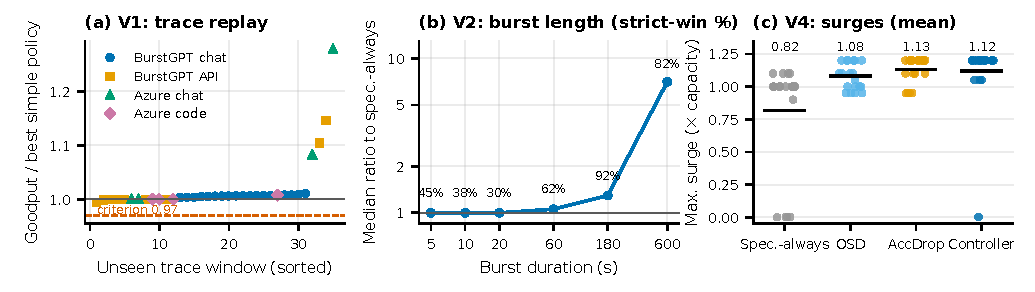
\includegraphics[width=\linewidth]{figures/fig5_heldout.pdf}
\caption{Frozen-simulator validation on unseen workloads. (a) Goodput of the controller relative to the best of five simple policies in each of \nv{v1.n} trace windows (sorted). (b) Median goodput relative to \pol{SpecAlways} for bursts of a new domain, by burst length; labels give the share of strict wins. (c) Largest surge, in multiples of plain-decoding capacity, served without SLO violation in 20 scenarios (dots) and their mean (bars).}
\label{fig:heldout}
\end{figure*}

The live runs cover one workload shape. To test other traffic, we replay traces in a simulator built from the same frozen calibration file: a fluid single-GPU model in which arrivals set the operating concurrency, excess demand queues, training slows serving by $\kappa(C)\,d$, and acceptance follows the measured learning curves, including the measured transfer to chat. The simulator implements the controller's rules, with goodput (tokens served within the SLO) instead of throughput as the currency under saturation, and five simple policies: \pol{NoSpec}, \pol{SpecAlways}, and three that keep speculation on and train at full duty when a trigger fires: \pol{OSD} (fewer than 16 running requests), \pol{Timed} (30\,s every 5 minutes), and \pol{AccDrop} (acceptance below 95\% of the ceiling, an acceptance-triggered rule in the spirit of TIDE). We froze the simulator and the calibration (hashes \texttt{\nv{sim.hash}} and \texttt{\nv{model.hash}}) and declared four criteria before running workloads never used in development: \nv{v1.n} trace windows from BurstGPT \citep{wang2024burstgpt} chat and API logs on days we had not replayed and from the Azure 2023 chat and code traces \citep{patel2024splitwise}, each at three or four load scales; 60 random bursts of a new domain; 40 Chinese regimes; and 20 surge scenarios at seven surge levels (\cref{app:sim}).

Figure~\ref{fig:heldout} and \cref{tab:heldout} in \cref{app:sim} report the outcomes. The goodput criterion holds in all \nv{v1.n} trace windows: the controller is never more than \nv{v1.short}\% below the best simple policy and is the best policy in \nv{v1.best}. It trains on \nv{v1.cmtrain.min}--\nv{v1.cmtrain.max}M tokens per trace window, whereas \pol{OSD} trains on up to \nv{v1.osdtrain.max}M; the training criterion fails only in four Azure chat windows, where \pol{OSD} itself trains on fewer tokens than the controller. Three expectations did not survive. First, training pays back reliably only for long bursts: short bursts are mostly ties, strict wins reach \nv{v2.d60.win}\% at 60\,s and \nv{v2.d180.win}\% at 180\,s. Second, the controller ranks above \pol{SpecAlways}, \pol{OSD}, and \pol{AccDrop} in all \nv{v3.n} Chinese regimes, but its advantage over \pol{SpecAlways} is \nv{v3.feas.min}--\nv{v3.feas.max}$\times$ at feasible saturation and as low as \nv{v3.over.min}$\times$ under overload, so the pre-declared $1.5\times$ margin fails. Third, \pol{AccDrop} tolerates surges as well as the controller (mean \nv{v4.acc} versus \nv{v4.cm}); the controller's advantage lies in meeting all four criteria at once. Finally, the horizon forecast barely matters in these workloads: replacing it with the true remaining length of the regime changes the outcome in \nv{hz.diff} of \nv{hz.total} cases.

\subsection{Overheads}\label{sec:overheads}

The export path and the trainer's memory reserve cost \nv{moe.infra}--\nv{code.infra}\% of phase-B throughput (\pol{Production} versus \pol{Static}). The engine's speculation-off state is \nv{zh.switch_vs_plain.abs}--\nv{code.switch_vs_plain.abs}\% slower than serving without a drafter. Part of the gap is the first seconds of phase B, which are served with speculation on; the rest is the cost of keeping the drafter loaded while speculation is off, which we did not separate further. It is the largest overhead and a target for engine work. Drafter swaps (\nv{swap.m1.min}--\nv{swap.m1.max}\,s for Qwen3-8B, \nv{swap.m2.min}--\nv{swap.m2.max}\,s for MoE) and speculation switches (at most \nv{switch.max}\,ms) did not cause a single failed request in the \nv{n.runs} runs (\cref{app:extra}).
